\begin{frame}{Why interpretability?}
\begin{columns}
\begin{column}{.33\textwidth}
\begin{figure}
    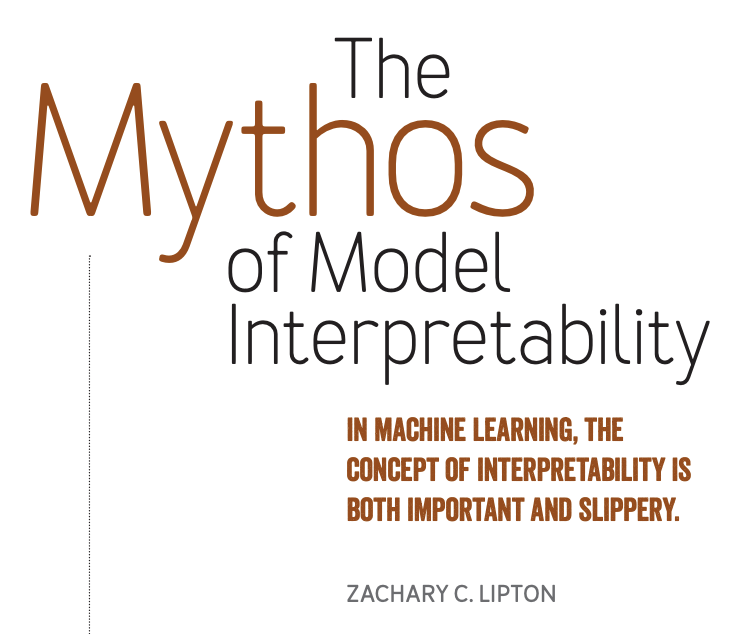
\includegraphics[width=4cm]{img/zipton.png}
\end{figure}
\begin{itemize}
    \item \citet{Molnar2023-le} is a great introduction to interpretability for neural networks
\end{itemize}
\end{column}
\begin{column}{.5\textwidth}
\begin{itemize}
    \item Sample efficiency: interpretable models can learn from less data and generalize better
    \item Safety: For language models, a common goal is to guarantee how a model will respond in a certain situation
    \item There is a distinction between post hoc model interpretability and inherently interpretable models
\end{itemize}
\end{column}
\end{columns}
\end{frame}

\begin{frame}[fragile]{Interpretability concepts}
\centering
\begin{figure}[H]
    \centering
\begin{tikzcd}[column sep=small]
 & \text{Data } \mathcal{D} \arrow[dl] \arrow[dr] & \\
\text{Embedding } \phi(\mathcal{D}) & &  \text{Dictionary } \mathcal{G} (\mathcal D) = \{c_1 \dots c_p\}
\end{tikzcd}
    \label{fig:summary}
\end{figure}
\begin{table}[H]
\scriptsize
\centering
\begin{tabular}{|c|p{3cm}|p{5cm}|}
\hline
\textbf{Concept} & \textbf{Definition} & \textbf{Example} \\
\hline
Data & Raw input data & Molecular dynamics coordinates, gene expression, language model tokens \\
Embedding & Potentially learned transformation & Projection into latent spaces of neural networks, Principal Component Analysis (PCA) results, UMAP results \\
Dictionary & Interpretable functions & Bond rotation, cell-cycle, luminosity \\
\hline
\end{tabular}
\label{tab:concept_examples}
\end{table}
\end{frame}


\begin{frame}[fragile]{Estimating interpretable representations}
Interpretability algorithms attempt automatic association $\mathcal D$ or $\phi(\mathcal D)$ with $\mathcal G (\mathcal D)$
\begin{columns}
\begin{column}{.5\textwidth}
\begin{itemize}
    \item Local Interpretable Model-agnostic Explanations \citep{Ribeiro2016-rm}
    \item Tangent Space Lasso \citep{Koelle2024-no}
\end{itemize}
\end{column}
\begin{column}{.5\textwidth}
\begin{figure}
    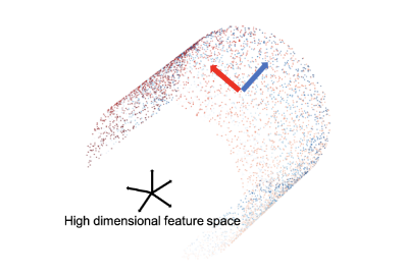
\includegraphics[width=5cm]{img/swisstangent.png}
    \caption*{The TSLasso approach - dictionary functions colored on the data manifold}
\end{figure}
\end{column}
\end{columns}
A large number of interpretability approaches are reviewed in \citet{Elhage-ob, Molnar2023-le}.
\end{frame}

\begin{frame}{Vector space representations}
\begin{itemize}
    \item It has been observed that (e.g. \citep{Mikolov2013-bs}) that neural networks create vector spaces of concepts in their latent space
\end{itemize}
\begin{align*}
    \phi("king") - \phi("man") + \phi("woman") = \phi("queen")
\end{align*}
\begin{itemize}
\item But, these concepts are often not basis aligned, and more concepts are represented than there are dimensions in the space.
\end{itemize}
\begin{figure}
    \centering
    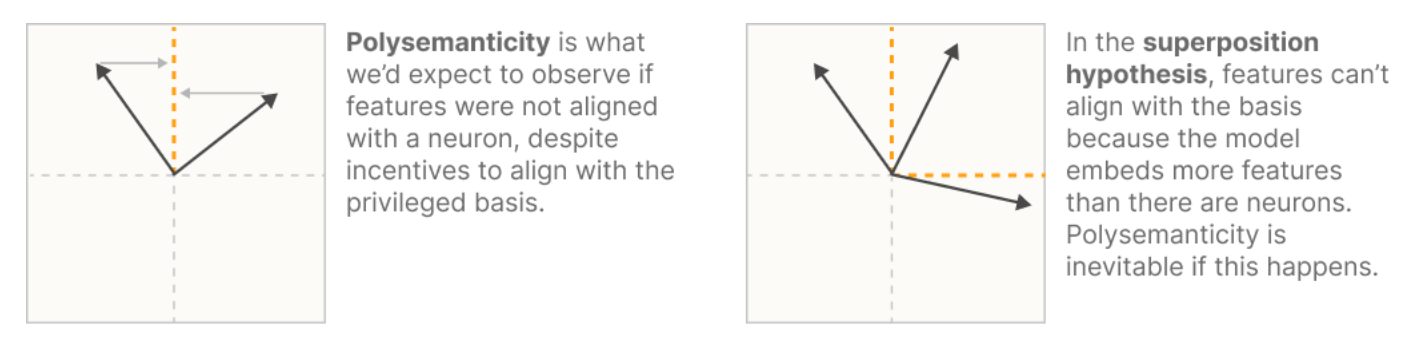
\includegraphics[width=8cm]{img/superposition.png}
    \caption*{\citet{Elhage-ob}: possible because of sparsity and noisy computation.}
    \label{fig:enter-label}
\end{figure}
\end{frame}

\begin{frame}[fragile]{Another view on interpretability}
\begin{itemize}
    \item The notion of interpretability research expounded in \citet{Cunningham2023-mu} comes from \citet{Elhage-ob}
    \item Functional independence in \citet{Koelle2024-no} = decomposibility
\end{itemize}
\begin{figure}
    \centering
    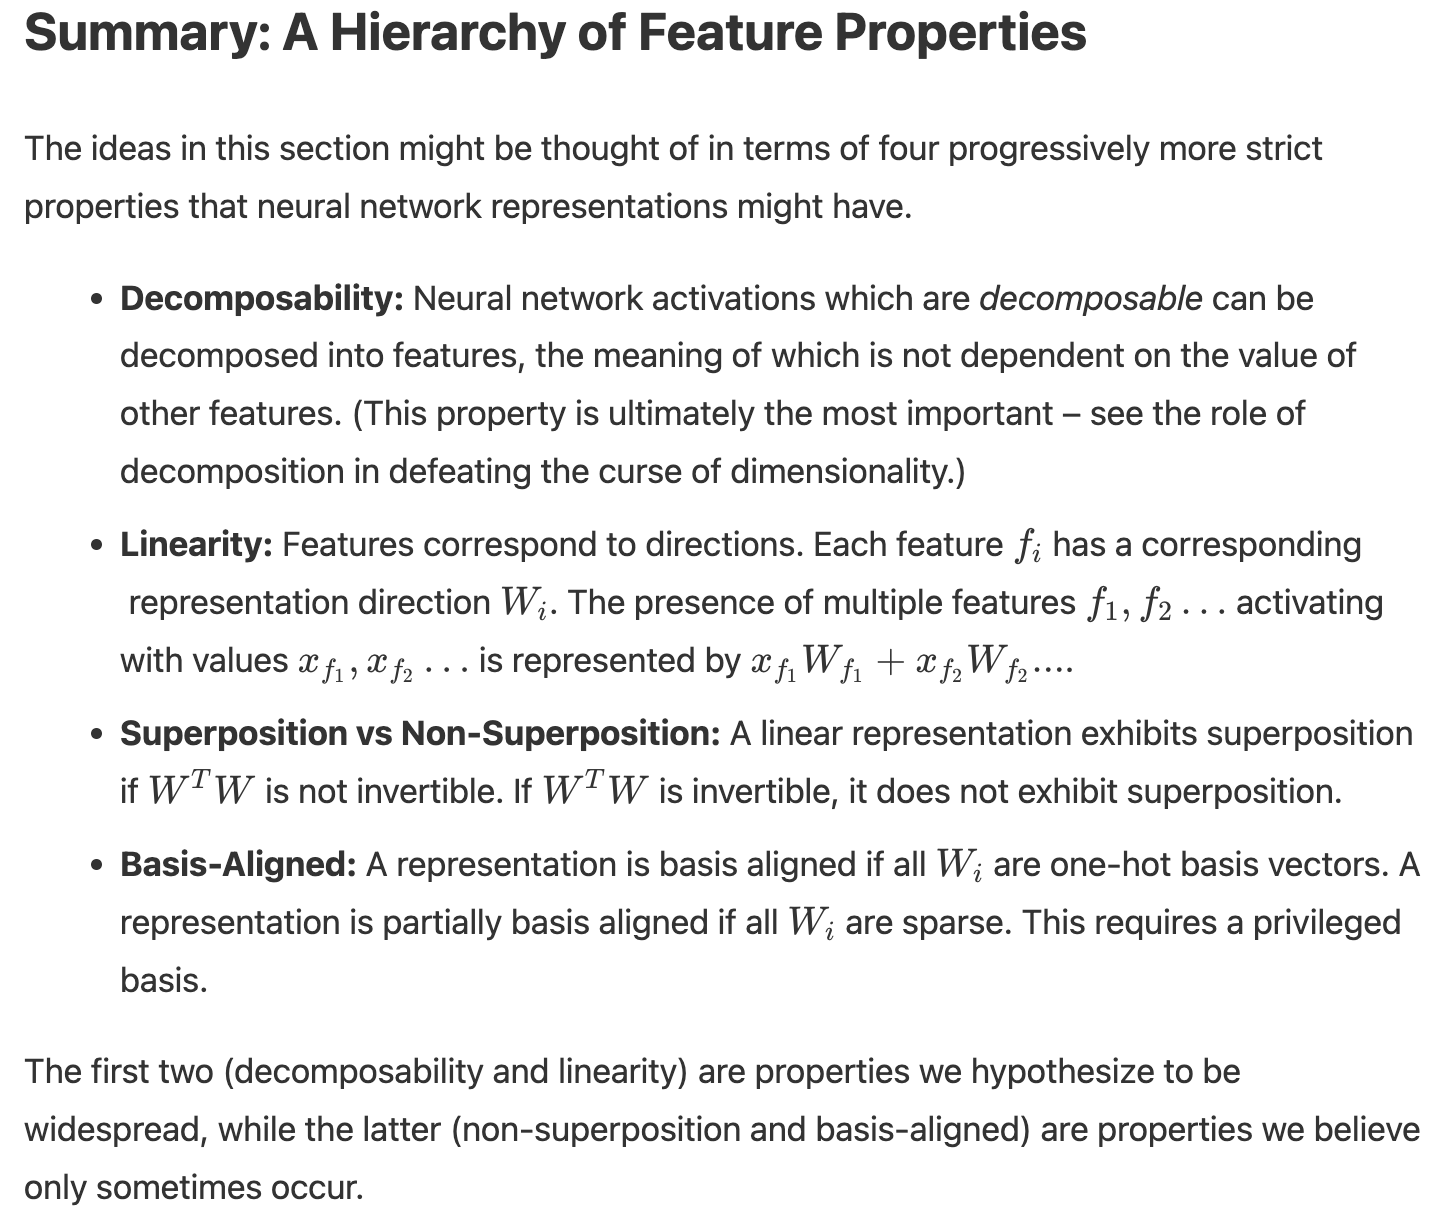
\includegraphics[width=6cm]{img/anthropicinterpretability.png}
    \caption*{Here, feature $=$ dictionary function.}
    \label{fig:enter-label}
\end{figure}
\end{frame}

\begin{frame}[fragile]{Constructing Dictionaries for Language Models}

\begin{itemize}
    \item One of the essential questions when considering interpretability w.r.t. a dictionary is what features should be in the dictionary
    \item A method for scoring features in language models is proposed by \citet{Bills-ec}.
    \item In this method, data points that have high values w.r.t. a particular feature $c_j$ are fed to an "explainer" model (GPT4)  that comes up with an explanation for the feature.
    \item That explanation is then used by an "interpretability scoring" model (GPT3.5) to predict feature values for held out data points.
    \item The idea is that simpler, more interpretable concepts will result in more accurate prediction.
    \item Summarized as interpretability score $\hat I (c_j) = \|c_j (h_i) - \hat c_j(h_i)\|$.
\end{itemize}
%\end{center}

\vspace{1em}
%\textbf{Why can we embed a whole concept at once?}
\end{frame}



